\documentclass{article}
\usepackage{graphicx}
\usepackage{titletoc}
\usepackage{titlesec}
\usepackage{geometry} 
\usepackage{fontspec, xunicode, xltxtra}
\usepackage{float}
\usepackage{cite}
\usepackage{amsmath}
\usepackage{listings}
\usepackage{titletoc}

\geometry{left=3cm,right=3cm,top=3cm,bottom=3cm}
\DeclareMathOperator*{\argmin}{argmin}
\DeclareMathOperator*{\argmax}{argmax}
\DeclareMathOperator*{\var}{var}
\DeclareMathOperator*{\expec}{E}

\begin{document}
\title{\textsf{Homework 2 for Pattern Recognition}}
\author{Fan JIN\quad (2015011506)}
\maketitle

\section*{Question 1}
{
    \subsection*{(1)}
    {
        The error function is minimized when optimized: 
        $$\frac{\partial}{\partial w_0} E(w, w_0) = \sum_{i=1}^{n} {(w^T x_i + w_0 - t_i)} $$
        $$= n w^T m + nw_0 + n_1 \frac{n}{n_1} + n_2 \frac{-n}{n_2} = n ( w^T m + w_0 ) = 0,$$
        which yields $$w_0 = -w^T m$$.
    }

    \subsection*{(2)}
    {
        Denote the observation matrix and the response matrix as 
        $$x = [x_1-m, x_2-m, \cdots, x_n-m]$$ and $$t = [t_1, t_2, \cdots, t_n].$$
        Plug in the optimal $w_0 = -w^T m$, and the error function can thus be expressed as 
        $$E(w) = \frac{1}{2} (w^T x - t)(w^T x - t)^T.$$

        By matrix calculus\footnote{See https://en.wikipedia.org/wiki/Matrix\_calculus}, we have
        $$\frac{\partial}{\partial w} E(w) = -x (t^T - x^T w) = 0,$$
        that is, $$x x^T w = x t^T.$$

        Note that $$x t^T = \left[ \sum_{i=1}^{n} {(x_i t_i)} \right] - m \cdot \sum_{i=1}^{n} {x_i} $$
        $$= \left[ \left(n_1 \frac{n}{n_1} m_1 + n_2 \frac{-n}{n_2} m_2 \right) \right] - m \cdot \left( n_1 \frac{n}{n_1} + n_2 \frac{-n}{n_2} \right) = n (m_1 - m_2),$$ and 
        $$m = \frac{n_1}{n}m_1 + \frac{n_2}{n}m_2 = m_1 - \frac{n_2}{n}(m_1-m_2) = m_2 + \frac{n_1}{n}(m_1-m_2),$$ we have
        $$x x^T = \sum_{i\in C_1}{(x_i - m_1 + \frac{n_2}{n}(m_1-m_2))(x_i - m_1 + \frac{n_2}{n}(m_1-m_2))^T} $$$$+ \sum_{i\in C_2}{(x_i - m_2 - \frac{n_1}{n}(m_1-m_2))(x_i - m_2 - \frac{n_1}{n}(m_1-m_2))^T}$$
        $$= \sum_{i\in C_1}{(x_i - m_1)(x_i - m_1)^T} + \sum_{i\in C_2}{(x_i - m_2)(x_i - m_2)^T} + \frac{n_1 n_2}{n^2} \sum_{i=1}^{n} {(m_1 - m_2)(m_1 - m_2)^T}$$
        $$= S_w + \frac{n_1 n_2}{n} S_B.$$

        Therefore, we proved that $$\left( S_w + \frac{n_1 n_2}{n} S_B \right) w = n (m_1 - m2)$$ when $w$ is optimal.

    }

    \subsection*{(3)}
    {
        Note that $$S_B w = (m_1 - m_2) (m_1 - m_2)^T w = (m_1 - m_2) \cdot \left[ (m_1 - m_2)^T w \right],$$ and that $(m_1 - m_2)^T w$ is a scalar. Therefore, the vector $S_B w$ is proportional to $m_1-m_2$, which means $$w \propto S_w^{-1} (m_1 - m_2).$$
    }
}

\section*{Question 2}
{
    \subsection*{Data Visualization}
    {
        Since the dimension of original data is high, we apply PCA (Principal Component Analysis) and extract the first two principal compenents for a scatter plot. 

        \begin{figure}[H]
            \centering
            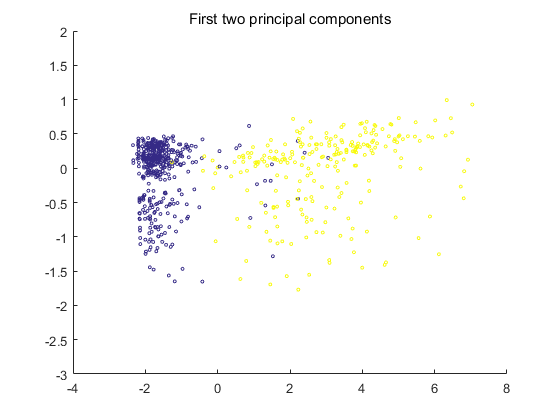
\includegraphics[width = 0.8\linewidth]{pca.png}
            \caption{Scatter plot}
        \end{figure}

        The data seems linearly separable, although there are a few outliers.
    }

    \subsection*{Logistic Regression}
    {
        I implement the algorithm on my own, using a loss function based on cross entropy
        $$L(\theta) = - \sum_{i} {\left[ y_i \log{(h_\theta (x_i))} + (1 - y_i) \log{(1 - h_\theta (x_i))}\right]},$$
        where $$h_\theta (x_i) = \frac{1}{1 + \exp{(- \theta^T x_i)}}.$$

        Gradient descent is employed to solve the optimal parameter $\theta$. A column of ones is attached to the data matrix, in order not to write the intercept in the expression.

        The error rate is $3.33\%$ on the validation set.

    }

    \subsection*{Fisher's Discriminant}
    {
        I implement the algorithm on my own, using the formula in Question 1.

        The error rate is $1.43\%$ on the validation set.

    }

    \subsection*{Discussion}
    {
        Why does the Fisher's method have better performance than logistic regression? 

        Their main difference is their loss functions. Logistic regression uses the cross entropy, while the Fisher's method adopts the ordinary quadratic loss, or the sum of squared errors (SSE). With outliers in consideration, the cross entropy tends to punish more on outliers, compared to the SSE loss function, and therefore, is more likely to result in over fitting.

        Another reason is that the Fisher's method considers the variance of two categories. It can predict the data distribution well if the positive samples have a variance different from that of the negative samples.

    }
}

\section*{Source Code}
{
    Please download the souece code from http://39.106.23.58/files/PR2\_2015011506.7z
}

\clearpage
\end{document}
    